\section{Заключение}
\begin{frame}
    \frametitle{Послесловие}
    \only<1->{
        Это был всего лишь обзорный взгляд на физику с точки зрения
        философствующего аспиранта.
    }
    \only<2->{
        \par\vspace{0.3cm}
        Настоящий вводный курс по механике должен состоять из пары лекций,
        пяти семинаров, и письменным и устным экзаменами в конце.
    }
    \only<3->{
        \par\vspace{0.3cm}
        Тем, кому интересно заниматься дальше: обратитесь ко мне, мы
        попробуем договориться с <<Абракадаброй>> и ТУМом.
    }
    \only<4->{
        \par\vspace{0.3cm}
        Заодно можно будет посмотреть на всякие интересные штуки в Гархинге
        или в Deutsches Museum.
    }
    \only<5->{
        \par\vspace{0.3cm}
        И хотелось бы мне вам рассказать про низкоуровневое
        программирование: как шаг за шагом конструируются современные
        компьютерные программы, начиная с уровня микрочипов.
    }
\end{frame}

\begin{frame}
    \frametitle{Спасибо за внимание!}
    \begin{figure}
        \begin{centering}
            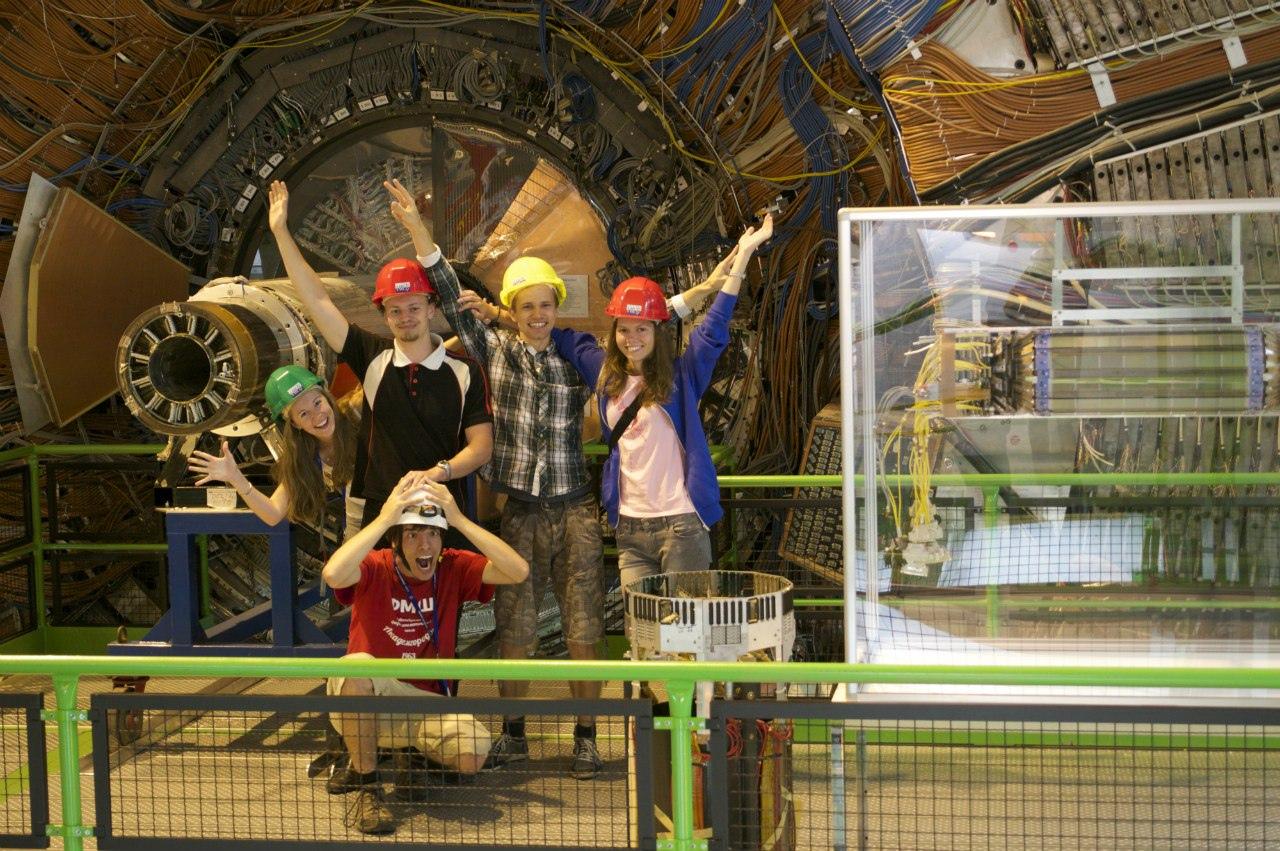
\includegraphics[width=0.7\textwidth]{summary}
        \end{centering}
    \end{figure}
\end{frame}

\begin{frame}
    \frametitle{Ссылки на источники}
    Публичная лекция В. Вахштайна <<Наука и искусство: самореференция и
    интервенция>>
    \par\vspace{0.3cm}
    Открытая группа CERN на facebook
    \par\vspace{0.3cm}
    Открытая группа Belle II на facebook
    \par\vspace{0.3cm}
    Материалы с \url{https://belle2.org}
    \par\vspace{0.3cm}
    Личные фотографии
\end{frame}
